% This version uses the latex2e styles, not the very ancient 2.09 stuff.
\documentclass[letterpaper,twocolumn,11pt]{article}
\usepackage{usenix,epsfig,endnotes}
\usepackage{hyperref}
\usepackage{framed}
\usepackage{caption}
\usepackage{float}
\usepackage{amsmath}



\begin{document}

%don't want date printed
\date{\today}

%make title bold and 14 pt font (Latex default is non-bold, 16 pt)
\title{\Large \bf  Link Prediction in Bipartite Graphs}

%for single author (just remove % characters)
\author{
{\rm Anirudh Narasimhamurthy}\\
u0941400\\ 
University Of Utah
\and
{\rm Soumya Smruti Mishra}\\
u0926085\\ 
University Of Utah
% copy the following lines to add more authors
% \and
% {\rm Name}\\
%Name Institution
} % end author

\maketitle

% Use the following at camera-ready time to suppress page numbers.

\thispagestyle{empty}

\subsection*{Abstract}
One of the challenges in network analysis is to predict what new connections will be created in the particular graph/network at some point in future. Many real world networks like user-products or user-business relations have a bipartite nature to them and evolve during time. Predicting links that will appear in them is one of the main approaches to understanding them. This was our main point of interest and we decided to understand link prediction problem in bipartite networks in our project. We also see how this can be extended or formulated to be applied to a recommendation problem. 


\subsection*{Classification Keywords}
link prediction, collaborative filtering, recommendation, bipartite graph,


\section{Motivation}
The primary motivation for selecting this project was based on two reasons: 
\begin{enumerate}
\item Firstly we wanted to explore and learn about link prediction and bipartite graphs. From our literature survey and reading papers \cite{two} \cite{six} \cite{seven} \cite{eight} we realized that link prediction in bipartite graphs was something which was less explored and hence we were interested to learn more about it through our project. 
\item Secondly we were also trying to see if we could use any of the Machine Learning techniques which we had learned about in this project and we believed the problem which we chose would probably help us in achieving it. 
\end{enumerate}

\section{Introduction}

\begin{itemize}
\item[] Link prediction is an important research problem in dynamic network analysis. Most of the problems which can be modeled as networks today are dynamic in nature i.e they evolve with node and link additions and removals. Typical examples include user - product relations where users are linked to the products they bought.


\item[] \cite{nine} states that social networks are not static and keep growing with time with addition of new nodes and links. Similarly user-product networks also evolve with time. This deals with link formation in the graphs i.e given nodes in a network the network grows by forming new relationships with existing nodes. We in this project deal with the question of predicting if a link will be formed between user and product/business.


\item[] Being able to predict such links accurately can have important implications in different networks including uses in national defense, predicting future credit card frauds and other related problems.Also a lot of the current research from what we understood focuses on link prediction on graphs with one type of node such as predicting links in social networks(Twitter, Facebook, LinkedIn) which is made up of people only. We wanted to explore methods which could be applied for a bipartite graph setting.


\item[] In this project we attempted to use our understanding of the concepts we learned in this course in line with different methods we came across the literature and used the following methods for link prediction in bipartite graph:
\begin{enumerate}
\item Similarity measures using Jaccard similarity and common neighbors
\item Approach based on completing the matrix entries using decomposition techniques
\item A page rank style approach using Random walks.
\item Supervised binary classification method.
\end{enumerate}
\end{itemize}

%After a new question is submitted in stackoverflow, most of them turn out to be invalid questions which are closed due to one of the following reasons: Off topic, not constructive, not a real question, too localized or exact duplicate. Hence, Kaggle posted a competition to use machine learning strategies to identify the best prediction model.



\section{Formal Problem Description}

Our project attempts to predict new links which can potentially be formed in a network in future, given a snapshot of the current network and to evaluate its effectiveness. We are also primarily involved in applying the different metric to bipartite graphs.


\section{Definitions}
Bipartite graph: A bipartite graph or bigraph is a set of graph vertices decomposed into two disjoint sets such that no two graph vertices within the same set are adjacent to each other.

\section{Assumptions}
\label{sec:assumptions}
\begin{enumerate}
\item One of the primary assumptions that we make is although collaborative filtering recommendation technique might work with the data set, our interest was to learn about link prediction in bipartite graphs and so we model our data set as bipartite graph.
\item Link prediction is our primary goal and recommendation is a side product of this one and we assume the recommendation or result which we state in our later sections might be a possible result although the sparsity and other factors might point otherwise.
\item Also for our data set without taking the location into consideration, we assume the prediction that we make is reasonable one although in practice there could be a lot of other things needed to make such a prediction.
\end{enumerate}

\section{Scope}

Our main stating is that the approaches used in our project could potentially be applied to a different data set which exists as or can be modeled as bipartite graph and even if the example data set which we have taken might not sufficiently convince that, we wanted to make it clear that our scope lies in the understanding of methods/measures which could be applied for link prediction in bipartite graphs. Results and other observations stated in later sections are our understanding but the bigger picture could or could not be different. 

\section{Prior Work}

\begin{itemize}

\item A lot of work has been done on link prediction in general.In \cite{four} they experiment with several similarity metrics including Graph Distance, Preferential attachment, Katz method and others. These could be modified so that they can be applied to bipartite graphs. In our project we experiment with two similarity metrics stated in Introduction section.

\item Link prediction in bipartite networks has not been explored extensively. In \cite{five} they describe how similarity metrics could be used as features in bipartite setting and they describe machine learning approaches to solving this problem. Supervised link prediction methods were also suggested.

\item Other works in bipartite link prediction include \cite{two, three}. In \cite{two} they use a kernel based approach to link prediction while \cite{three} uses a different distance metric approach.

\item One of the co-authors of our prescribed text book Jure Leskovec has also done research in this area and in \cite{one} they propose a random walk approach to link prediction which makes use of both a distance metric and Page Rank style approach.

\item Our approaches used in our project are primarily influenced by the above mentioned works.

\end{itemize}

\section{Data}

\subsection{Dataset used for the Project}
We used the TripAdvisor dataset for our project. It was obtained from Database and Information Systems Laboratory of University of Illinois, Urbana Champaign from the following url \url{http://times.cs.uiuc.edu/~wang296/Data/}

\subsection{Dataset description}
The raw dataset consisted of set of reviews written by different users for different hotels along with the ratings given by the user to different aspects of the hotel. Every review also had a date associated with it. The date range for the reviews in the dataset was from 2002 till 2012. The size of the dataset was 2.06 GB. A snapshot of a the raw review data is shown below for better understanding:


\begin{figure}[H]
\begin{center}
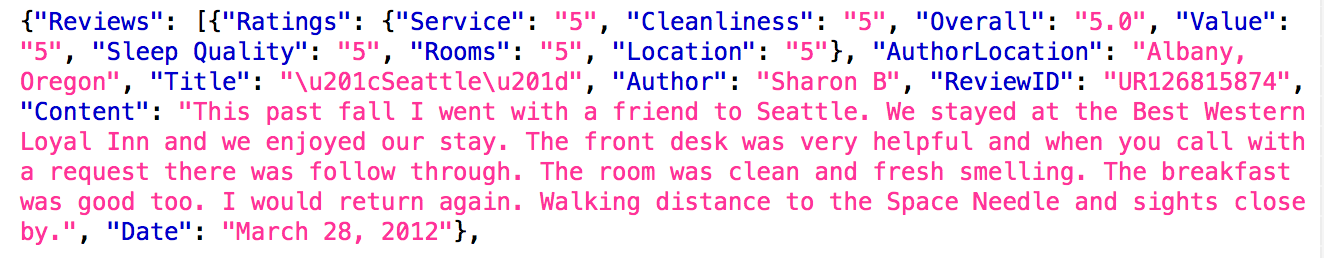
\includegraphics[width=1\linewidth]{images/raw_data.png}
\captionof{figure}{Raw review data}
\label{fig:status}
\end{center}
\end{figure}


\subsection{Data processing}
The most important aspect of our problem is to model the given dataset as a bipartite graph. From the definition mentioned earlier, to model the given data as a bipartite graph, the following processing was required to be done:

\begin{itemize}
\item In order to lessen the load on our processing we removed the review text from all the files and then created a cleaned up reviews.json. We adopted this approach with the assumption that we would not be making use of review content to do a prediction. The cleaned up reviews file had the following fields

\begin{enumerate}
\item Ratings
\item Author name or User name
\item Author Location
\item Date of Review
\item HotelID
\item Hotel Location
\end{enumerate}

\item Using the reviews.json created in the above step, we then created two more files one for users/authors and the other for hotels. The users.json had the following fields:
\begin{enumerate}
\item AuthorID ( a unique ID assigned by us)
\item ReviewCount (aggregation of all the reviews written by this author identified by Name/ID)
\item Last Review Date( date of the last review written by this author/user)
\item UserLocation
\end{enumerate}

\item The hotels.json file on the other hand had the following fields:
\begin{enumerate}
\item HotelID
\item ReviewCount (aggregation of all the reviews written for this Hotel identified by ID)
\item HotelLocation
\end{enumerate}

\item At the end of this processing, the count of hotels and users are given below:
\begin{table}[h]
	\centering
	\begin{tabular}{ |p{3cm}|p{3cm} |}
		\hline
		Hotels count	&	11797\\  \hline
		Users count  &	781237 \\  \hline
		
	\end{tabular}
	\caption{Hotels and users count} 
	\label{tab:dist1} 
\end{table} 

\item These two files users.json and hotels.json would then help us model the bipartite graph as we would have all the users on one side of the graph and we would have all the hotels on the other side of the graph and an edge goes between user and hotel if a user has written a review  for that hotel.

\item As stated earlier that prediction will be done based on the snapshots of the network or graph created at different times. We used t(training) as Jan 1, 2013 meaning all data before it and t'(test) as Jul 1,2013  meaning all data between t and t' to create train and test data respectively. To get the required graph in terms of nodes and edges,we had to do further processing.

\item From the hotels and users file, we picked out the IDs and then assigned a unique ID for each of the HotelID and UserID which is a running sequence so that there is better clarity when we look at the graph data file. Once IDs were created we then created the graph.txt file for both test and train data which will contain all the edges in the current dataset represented by nodes on either side.

\item Once we created graph.txt to get statistics about the graph, we used some of the built in methods from SNAP.py package and also referred to code blocks online to get the following details:
\begin{table}[ht]
	\begin{tabular}{ |p{5cm}|p{2cm} |}
		\hline
		\textbf {Property} & \textbf{Value}\\ \hline
		Number of nodes	&	793034 \\  \hline
		Number of edges	&	1088791 \\  \hline
		IsConnected	&	No \\  \hline
		Average Degree of a node		&	1.372944\\  \hline

		
	\end{tabular}
	\caption{Statistics on the graph.txt} 
	\label{tab:dist} 
\end{table} 

\end{itemize}

\subsection{Creating examples from input data}

We also wanted to experiment with supervised learning methods for link prediction and hence we had to create examples so that it could be used by our classifier to predict the output. During the creation of examples, we did a further filtering to ensure data is not overly skewed and it is at an acceptable level. This idea was obtained from one of the projects of the Stanford Data Mining Class handled by Jure Leskovec. The following filtering was done:

\begin{enumerate}
\item Only taking users who have been active in the last six months. To do this we made use of the Last Review Date field which we had included while creating users.json.

\item Only taking hotels which are at a distance 3 or 3 hop distance from current user as candidate edges. To compute the hop distance we made use of methods in SNAP.py package
\end{enumerate}

For creating examples we again made use of graph.txt as the input and also took data snapshots at two different times t and t' to create train and test examples.

The way users review hotels evolves over time and so test and training may have huge differences but we assume that those differences would be small enough that supervised learning would still be effective. We try to see if that is the case. Furthermore we felt it was justified in the sense even in real world scenario this is how data would probably end up being because we would have information only about the previous links.

\subsection { Statistics on examples and positive negative stuff}

$<<<<<<<<<<<<< $TO BE COMPLETED \\
I did not understand what is being done there. But I realize it is important for the supervised learning part. So please kindly fill in your understanding and then tell what those values represent \\
Also\\
describe\\
about \\
the\\
matrix.json file\\
and \\
edges.txt\\
which gets created\\
in this \\
section\\
I don't understand \\
what \\
they are\\
doing\\

$>>>>>>>>>>>>>>>>>>>>>>$


\section{Similarity Measures for Link Prediction in Bipartite Graphs}

\begin{itemize}

\item Similarity metrics can be used to compute the score of each candidate edge or potential links which might appear in future.

\item Metrics used in \cite{four} compare the neighbors of two nodes in the edge. But to make it for bipartite graphs we have to modify it. Because of the property of bipartite graphs nodes on the same side or neighbors of nodes on opposite sides do not intersect. Hence we would want to model them in such a way that we have both sets of nodes to contain the same type of node i.e users/ hotels.

\item To do this, we choose two sets S(x) and S(y) for our similarity metrics given nodes(x,y) on opposite sides of a graph. We define S(x) and S(y) in a way which is similar to how we used hop distances for creating examples.

\begin{itemize}
\item S(x) represents nodes which are 2 hops away from x. Effectively this produces nodes on same side of the network as x because traveling two hops would be equivalent to going to x's neighbor and then coming back again to the same side of x. 

\item S(y) represents y's neighbors. These represent nodes on opposite side of y, which is nothing but same side of x, because we have modeled the graph as bipartite in this case.
\end{itemize}

\item To compute 2 hop distance we used SNAP package's GetNodesAtHop() method to get our required values. Also SNAP modules other methods for graph processing proved useful. We found this package to be useful when we were stumbling across different datasets in our initial search for project datasets.

\item Both the sets from the description above will comprise of node's on the side of x.  This enables us to use them to compute distance metrics. We used two such metrics in our project:

\end{itemize}

\subsection{Jaccard Similarity}

Jaccard Similarity is one of the widely and most commonly used similarity metrics. Jaccard similarity for our bipartite case is defined by:\\
$\frac {| S(x) \cap S(y) |}{| S(x) \cup S(y) |}$ \\

Jaccard similarity has the advantage that it is relatively easier to implement and also it is computationally less expensive than say cosine similarity for the same graph.

\subsection{Common Neighbors}
Common neighbors is a metric which is commonly used in graph networks where similarity could be measured in terms of the neighbors. For the bipartite case, it is simply defined as :\\
$|S(x) \cap S(y)|$


\subsection{Note}
 \begin{itemize}
 \item For the similarity measures we tried implementing using both the nodes as S(x) in the sense, we had S(x) as users and then calculated all the hotel's neighbors and we also considered S(x) as hotels and then calculated all user's neighbors for S(y)
 \end{itemize}

\subsection{Intuition behind similarity metrics and link prediction}

\begin{itemize}
\item Computing similarity metrics over these set of nodes is effective for link prediction because S(x) returns nodes which are similar to x since they are 2 hops away and on same side of x.

\item In other words users who review hotels that you do are likely to be similar to you. It is also reasonable to further assume if lot of them review the same hotel and there is a large overlap between them and s(x) then you are also likely to review that hotel in future. This in a way helps us to uncover the new links which might appear in the graph in future which is our primary motive.

\item As stated in the first, this is an assumption which we make and think is reasonable although it has been pointed out that this isn't so straightforward. But the bigger picture from this is, we learnt how to modify existing similarity metrics to be applied to a bipartite case, which was our primary goals.

\end{itemize}

\section{Random walk approach to Link Prediction}

In this section we describe how random walks can be used for link prediction in bipartite graphs.

\subsection{Definition}
A random walk is a finite Markov chain that moves through a graph G=(V,E)

\subsection{Ideas used from the class/course material}
\begin{itemize}

\item Suppose each edge/link in the given bipartite graph is assigned a weight w(u,v). Then based on the random surfer which we used for PageRank implementation, each edge (u,v) can also be assigned a transition probability $M_{u,v} =w(u,v) / d(u)$ where d(u)= $\sum_{(u,v) \epsilon E} w(u,v)$ is the weighted degree  of u or the number of outlinks from u.

\item These transition probabilities can be used  in random traversal of the graph  and when we run this process for a long time, it would eventually point to which nodes we might tend to visit. This in effect would tell us which hotel a user would likely review because an edge/link would be created based on the random walk's completion.

\item Convergence in this case would be slightly different from page rank case and also the transition probabilities at a stationary state would be given by $p_s= p_s M$
 \end{itemize}

\subsection{Description and Implementation}
\begin{itemize}
\item We used random walks to produce a score for each candidate edge (u,v). We scored the edge with the stationary distribution probability of reaching v when running a random walk from u.

\item To assign the weight to edges stated in the previous subsection, we found there were supervised methods of learning the weights and then applying them or using heuristics to decide the weight.

\item We preferred the approach which was simpler to us which was using heuristically chosen edge weights. In this case higher weights should be assigned to links which are likely to be more relevant. Relevance in our case would be the fact that the reviews written recently would tend to be a good reflection than a review which was written several years ago (for most cases and it is an assumption we make). This goes back to the point that as years go by people evolve and hotels evolve too and so the recently written reviews are likely to give a more accurate picture.

\item To take that into consideration we give each edge a weight of $w_{uv}$ =1/(c+$a_{uv}$) where $a_{uv} $is the age or the difference between current date and date of last review written by the user and c is a constant. 

\item We made use of methods available in networkx package in python for constructing adjacency matrix and scipy and numpy packages for other processing.

\item We used sc.parallelize() to create RDDs and used simple map reduce operations similar to our block matrix vector multiplications to calculate the probabilities and wrote the results to a json file.

\end{itemize}

\section{Low rank approximation technique to Link Prediction}

\begin{itemize}
\item As stated earlier in the context of a adjacency matrix, link prediction can be viewed as predicting new entries in the matrix of the graph. Again there might be issues with this approach given sparsity of the graph and the fact that absence of an entry in the matrix might not necessarily be interpreted as 0 in the boolean case. 

\item We weren't entirely sure of how the results would turn out but wanted to see what would be the results given this generic assumption and hence proceeded with it.

\item A commonly used technique for analyzing large matrices is to compute a low rank approximation for the given matrix. Different techniques are available for decomposition and we tried two of it:
\end{itemize}

\subsection{Singular Value Decomposition}

We tried to implement SVD for our given graph and then take the diagnol values to predict the potential links. The feedback given to us was to first try and do a SVD in say MATLAB and plot the diagnol entries of S. We tried that, but the size of the graph was so huge (1169456 x2) that a full adjacency matrix would exceed the maximum array size preference in MATLAB. 

To get an idea of the plot, we took the first 30000 entries and loaded into MATLAB and computed SVD just to get a rough idea of the plot. This might not be the correct approach but we wanted to make sure we did try the methods suggested in the feedback. The plot of diagonal  of the S matrix is shown below:


\begin{figure}[H]
\begin{center}
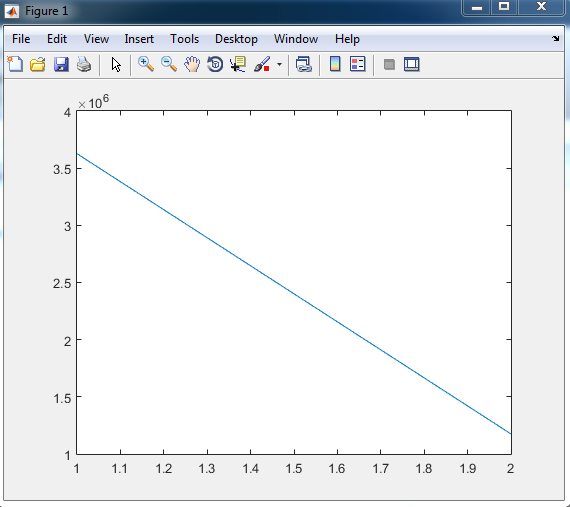
\includegraphics[width=1\linewidth]{images/SVD_output.png}
\captionof{figure}{Plot of diagonal of S matrix(30,000 entries)}
\label{fig:status}
\end{center}
\end{figure}

\begin{itemize}
\item The plot doesn't have the typical curve like the one which we have for collaborative filtering and hence might not be a good method to apply. Our data in graph.txt is in such a way that it probably makes this approach not suitable for this data.

\item Most of the diagonal entries were zero. This might either be due to the bipartite nature of the graph since edges can't go between nodes on the same side of the graph or it could be that this approach is not correct for this dataset. We weren't entirely sure and from the feedback that we got, we felt this was probably not the correct approach for this dataset.
 
\item But one of the reasons why we wanted to explore this approach was the fact for bipartite graphs, the adjacency matrices is symmetric and it would help with the processing where instead of going for the full adjacency matrix we could have used the sparse matrix for SVD computation.

\item We even tried experimenting with SVD in python using linalg package with the above approach and setting a value for k but we don't publish them in final results.

\item We also tried using the code for UV decomposition using Stochastic Gradient Descent available on the course website, but we weren't able to comprehend and didn't have much clarity with that.
\end{itemize}


\section{Supervised Binary Classifier approach to Link Prediction}
%Results (or for theoretical project, proofs)

\section{ Results and Evaluation}

\section{Conclusion}

\section{Difficulties faced in implementation}
\begin{enumerate}

\item 
\item 
\item 
\item 
\end{enumerate}


\section{Future Work}
%If you had much more time, how would you continue the project?

\begin{itemize}
\item 
\item 
\item
\item 
\end{itemize}



\bibliographystyle{plain}
\begin{thebibliography}{100}
	\bibitem{one} Lars Backstrom , Jure Leskovec, Supervised random walks: predicting and recommending links in social networks, Proceedings of the fourth ACM international conference on Web search and data mining, February 09-12, 2011, Hong Kong, China.   
    \bibitem{two} J. Kunegis, E. De Luca, and S. Albayrak. The link prediction problem in bipartite networks. In Computational Intelligence for Knowledge-Based Systems Design. 2010.
	\bibitem{three} Y. Yamanishi. Supervised bipartite graph inference. In NIPS, D. Koller, D. Schuurmans, Y.Bengio, and L. Bottou, Eds. MIT Press, 2008, pp. 18411848.
    
    \bibitem{four} Liben-Nowell, David and Kleinberg, Jon, The link-prediction problem for social networks,Journal of the American Society for Information Science and Technology,http://dx.doi.org/10.1002/asi.20591,2007.

    \bibitem{five} N. Benchettara, R. Kanawati, C. Rouveirol. Supervised Machine Learning applied to Link Prediction in Bipartite Social Networks. In Proceedings of the International Conference on Advances in Social Network Analysis and Mining. IEEE, Los Alamitos, CA, 326-330, 2010
    
   \bibitem{six} O. Allali, C. Magnien and M. Latapy , "Link prediction in bipartite graphs using internal links and weighted projection" ,  NetSciCom , pp.953 -958 
   
   \bibitem{seven} Xin Li , Hsinchun Chen, Recommendation as link prediction: a graph kernel-based machine learning approach, Proceedings of the 9th ACM/IEEE-CS joint conference on Digital libraries, June 15-19, 2009, Austin, TX, USA
   
   \bibitem{eight} Zan Huang , Xin Li , Hsinchun Chen, Link prediction approach to collaborative filtering, Proceedings of the 5th ACM/IEEE-CS joint conference on Digital libraries, June 07-11, 2005, Denver, CO, USA 
    
    \bibitem{nine} https://www3.nd.edu/~dial/papers/ICDM12b.pdf
    
    \bibitem{ten} F. Pedregosa, G. Varoquaux, A. Gramfort, V. Michel, B. Thirion, O. Grisel, M. Blondel, P.
Prettenhofer, R. Weiss, V. Dubourg, J. Vanderplas, A. Passos, D. Cournapeau, M. Brucher, M.
Perrot, and E. Duchesnay. Scikit-learn: Machine Learning in Python. In Journal of Machine
Learning Research, 12:2825-2830.
    
\end{thebibliography}



\end{document}